 \let\negmedspace\undefined
\let\negthickspace\undefined
\documentclass[journal]{IEEEtran}
\usepackage[a5paper, margin=10mm, onecolumn]{geometry}
%\usepackage{lmodern} % Ensure lmodern is loaded for pdflatex
\usepackage{tfrupee} % Include tfrupee package

\setlength{\headheight}{1cm} % Set the height of the header box
\setlength{\headsep}{0mm}     % Set the distance between the header box and the top of the text

\usepackage{gvv-book}
\usepackage{gvv}
\usepackage{cite}
\usepackage{amsmath,amssymb,amsfonts,amsthm}
\usepackage{algorithmic}
\usepackage{graphicx}
\usepackage{textcomp}
\usepackage{xcolor}
\usepackage{txfonts}
\usepackage{listings}
\usepackage{enumitem}
\usepackage{mathtools}
\usepackage{gensymb}
\usepackage{comment}
\usepackage[breaklinks=true]{hyperref}
\usepackage{tkz-euclide} 
\usepackage{listings}
% \usepackage{gvv}                                        
\def\inputGnumericTable{}                                 
\usepackage[latin1]{inputenc}                                
\usepackage{color}                                            
\usepackage{array}                                            
\usepackage{longtable}                                       
\usepackage{calc}                                             
\usepackage{multirow}                                         
\usepackage{hhline}                                           
\usepackage{ifthen}
\usepackage{lscape}
\begin{document}

\bibliographystyle{IEEEtran}



\title{2.5.20}
\author{EE25BTECH11057 - Rushil Shanmukha Srinivas
}
% \maketitle
% \newpage
% \bigskip
{\let\newpage\relax\maketitle}

\renewcommand{\thefigure}{\theenumi}
\renewcommand{\thetable}{\theenumi}
\setlength{\intextsep}{10pt} % Space between text and floats

\numberwithin{equation}{enumi}
\numberwithin{figure}{enumi}
\renewcommand{\thetable}{\theenumi}


\textbf{Question} : 
Let $\vec a,\vec b,\vec c$ be three vectors with $\lVert \vec a\rVert=1,\ \lVert\vec b\rVert=2,\ \lVert\vec c\rVert=3$. 
If the projection of $\vec b$ on $\vec a$ equals the projection of $\vec c$ on $\vec a$, and $\vec b\perp\vec c$, find
\begin{align}
\bigl\lVert 3\vec a-2\vec b+2\vec c\bigr\rVert.
\end{align}

\bigskip

\textbf{Solution (matrix / rank style).} :
Let us denote the scalar products
\begin{align}
x=\vec a\cdot\vec b,\qquad y=\vec a\cdot\vec c,\qquad z=\vec b\cdot\vec c .
\end{align}
Given: projection of $\vec b$ on $\vec a$ equals projection of $\vec c$ on $\vec a$.
Since $\lVert\vec a\rVert=1$, this implies
\begin{align}
\vec a\cdot\vec b=\vec a\cdot\vec c \quad\Rightarrow\quad x=y.
\end{align}
Also $\vec b\perp\vec c\Rightarrow z=0$. Using the magnitudes,
\begin{align}
\vec a\cdot\vec a=1,\quad \vec b\cdot\vec b=4,\quad \vec c\cdot\vec c=9.
\end{align}

Form the Gram (inner-product) matrix of $(\vec a,\vec b,\vec c)$:
\begin{align}
G=\myvec
{\vec a\cdot\vec a & \vec a\cdot\vec b & \vec a\cdot\vec c\\
\vec b\cdot\vec a & \vec b\cdot\vec b & \vec b\cdot\vec c\\
\vec c\cdot\vec a & \vec c\cdot\vec b & \vec c\cdot\vec c}
=
\myvec
{1 & x & x\\
x & 4 & 0\\
x & 0 & 9}
,
\end{align}
where we used $x=y$ and $z=0$.

Now denote the coefficient vector of $3\vec a-2\vec b+2\vec c$ relative to $(\vec a,\vec b,\vec c)$ by
\begin{align}
\mathbf{u}=\myvec {3\\-2\\2}.
\end{align}
Then the squared norm is the quadratic form
\begin{align}
\bigl\lVert 3\vec a-2\vec b+2\vec c\bigr\rVert^2
= \mathbf{u}^\top G\,\mathbf{u}.
\end{align}

\begin{align}
\mathbf{u}^\top G\, \mathbf{u}
=\myvec
{3 & -2 & 2}
\myvec
{1 & x & x\\
x & 4 & 0\\
x & 0 & 9}
\myvec 
{3\\-2\\2 }
=9 -6x +16 +6x +36 =61
\end{align}

Therefore
\begin{align}
\bigl\lVert 3\vec a-2\vec b+2\vec c\bigr\rVert^2 = 61
\quad\Longrightarrow\quad
\boxed{\bigl\lVert 3\vec a-2\vec b+2\vec c\bigr\rVert=\sqrt{61}}.
\end{align}
\pagebreak
\begin{figure}[h!]
  \centering
  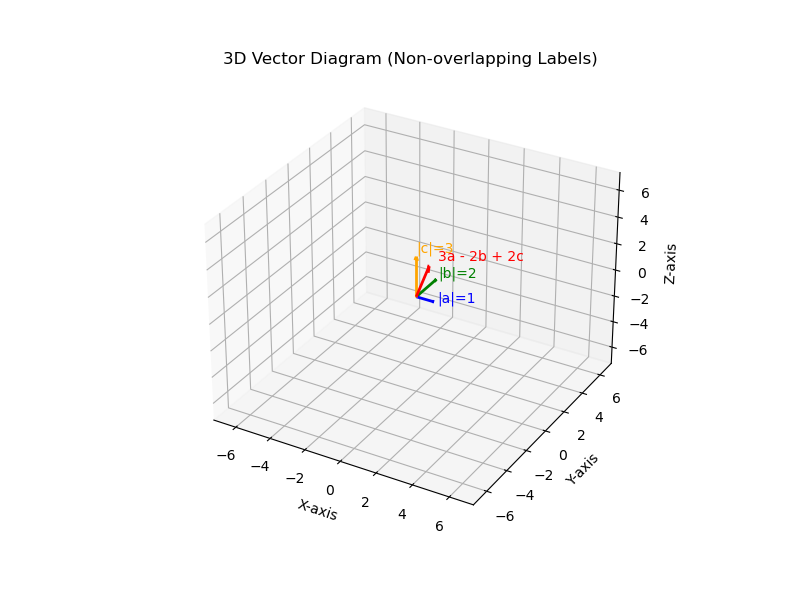
\includegraphics[width=0.9\columnwidth]{figs/fig3.png} 
   \caption*{Fig: Representation of vectors}
  \label{Fig3}
\end{figure}

\end{document}
